\chapter[On the Use of the tufte-book Document Class]{On the Use of the \texttt{tufte-book} Document Class}
\label{ch:tufte-book}

The \TL document classes define a style similar to the style Edward Tufte uses in his books and handouts. Tufte's style is known for its extensive use of sidenotes, tight integration of graphics with text, and well-set typography. This document aims to be at once a demonstration of the features of the \TL document classes and a style guide to their use.

%------------------------------------------------

\section{Page Layout}\label{sec:page-layout}
\subsection{Headings}\label{sec:headings}\index{headings}
This style provides \textsc{a}- and \textsc{b}-heads (that is, \Verb|\section| and \Verb|\subsection|), demonstrated above.

If you need more than two levels of section headings, you'll have to define them yourself at the moment; there are no pre-defined styles for anything below a \Verb|\subsection|. As Bringhurst points out in \textit{The Elements of Typographic Style},\cite{Bringhurst2005} you should ``use as many levels of headings as you need: no more, and no fewer.''

The \TL classes will emit an error if you try to use \linebreak\Verb|\subsubsection| and smaller headings.

\newthought{In his later books},\cite{Tufte2006} Tufte starts each section with a bit of vertical space, a non-indented paragraph, and sets the first few words of the sentence in \textsc{small caps}. To accomplish this using this style, use the \doccmddef{newthought} command:
\begin{docspec}
\doccmd{newthought}\{In his later books\}, Tufte starts\ldots
\end{docspec}

%------------------------------------------------

\section{Sidenotes}\label{sec:sidenotes}
One of the most prominent and distinctive features of this style is the extensive use of sidenotes. There is a wide margin to provide ample room for sidenotes and small figures. Any \doccmd{footnote}s will automatically be converted to sidenotes.\footnote{This is a sidenote that was entered using the \texttt{\textbackslash footnote} command.} If you'd like to place ancillary information in the margin without the sidenote mark (the superscript number), you can use the \doccmd{marginnote} command.\marginnote{This is a margin note. Notice that there isn't a number preceding the note, and there is no number in the main text where this note was written.}

The specification of the \doccmddef{sidenote} command is:
\begin{docspec}
\doccmd{sidenote}[\docopt{number}][\docopt{offset}]\{\docarg{Sidenote text.}\}
\end{docspec}

Both the \docopt{number} and \docopt{offset} arguments are optional. If you provide a \docopt{number} argument, then that number will be used as the sidenote number. It will change of the number of the current sidenote only and will not affect the numbering sequence of subsequent sidenotes.

Sometimes a sidenote may run over the top of other text or graphics in the margin space. If this happens, you can adjust the vertical position of the sidenote by providing a dimension in the \docopt{offset} argument. Some examples of valid dimensions are:
\begin{docspec}
\ttfamily 1.0in \qquad 2.54cm \qquad 254mm \qquad 6\Verb|\baselineskip|
\end{docspec}
If the dimension is positive it will push the sidenote down the page; if the dimension is negative, it will move the sidenote up the page.

While both the \docopt{number} and \docopt{offset} arguments are optional, they must be provided in order. To adjust the vertical position of the sidenote while leaving the sidenote number alone, use the following syntax:
\begin{docspec}
\doccmd{sidenote}[][\docopt{offset}]\{\docarg{Sidenote text.}\}
\end{docspec}
The empty brackets tell the \Verb|\sidenote| command to use the default sidenote number.

If you \emph{only} want to change the sidenote number, however, you may completely omit the \docopt{offset} argument:
\begin{docspec}
\doccmd{sidenote}[\docopt{number}]\{\docarg{Sidenote text.}\}
\end{docspec}

The \doccmddef{marginnote} command has a similar \docarg{offset} argument:
\begin{docspec}
\doccmd{marginnote}[\docopt{offset}]\{\docarg{Margin note text.}\}
\end{docspec}

%------------------------------------------------

\section{References}
References are placed alongside their citations as sidenotes, as well. This can be accomplished using the normal \doccmddef{cite} command.\sidenote{The first paragraph of this document includes a citation.}

The complete list of references may also be printed automatically by using the \doccmddef{bibliography} command. (See the end of this document for an example.) If you do not want to print a bibliography at the end of your document, use the \doccmddef{nobibliography} command in its place. 

To enter multiple citations at one location,\cite[-3\baselineskip]{Tufte2006,Tufte1990} you can provide a list of keys separated by commas and the same optional vertical offset argument: \Verb|\cite{Tufte2006,Tufte1990}|. 
\begin{docspec}
\doccmd{cite}[\docopt{offset}]\{\docarg{bibkey1,bibkey2,\ldots}\}
\end{docspec}

%------------------------------------------------

\section{Figures and Tables}\label{sec:figures-and-tables}
Images and graphics play an integral role in Tufte's work. In addition to the standard \docenvdef{figure} and \docenvdef{tabular} environments, this style provides special figure and table environments for full-width floats.

Full page--width figures and tables may be placed in \docenvdef{figure*} or \docenvdef{table*} environments. To place figures or tables in the margin, use the \docenvdef{marginfigure} or \docenvdef{margintable} environments as follows (see figure~\ref{fig:marginfig}):

\begin{marginfigure}
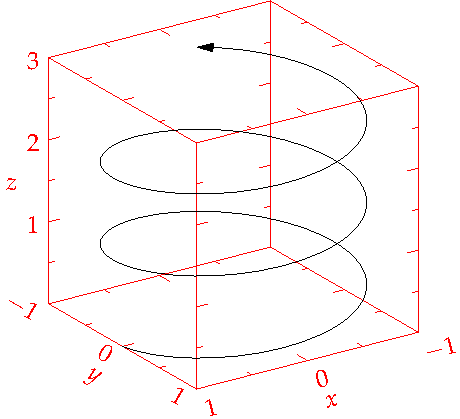
\includegraphics[width=\linewidth]{helix}
\caption{This is a margin figure. The helix is defined by $x = \cos(2\pi z)$, $y = \sin(2\pi z)$, and $z = [0, 2.7]$. The figure was drawn using Asymptote (\url{http://asymptote.sf.net/}).}
\label{fig:marginfig}
\end{marginfigure}

\begin{docspec}
\textbackslash begin\{marginfigure\}\\
\qquad\textbackslash includegraphics\{helix\}\\
\qquad\textbackslash caption\{This is a margin figure.\}\\
\qquad\textbackslash label\{fig:marginfig\}\\
\textbackslash end\{marginfigure\}\\
\end{docspec}

The \docenv{marginfigure} and \docenv{margintable} environments accept an optional parameter \docopt{offset} that adjusts the vertical position of the figure or table. See the ``\nameref{sec:sidenotes}'' section above for examples. The specifications are:
\begin{docspec}
\textbackslash{begin\{marginfigure\}[\docopt{offset}]}\\
\qquad\ldots\\
\textbackslash{end\{marginfigure\}}\\
\mbox{}\\
\textbackslash{begin\{margintable\}[\docopt{offset}]}\\
\qquad\ldots\\
\textbackslash{end\{margintable\}}\\
\end{docspec}

Figure~\ref{fig:fullfig} is an example of the \docenv{figure*} environment and figure~\ref{fig:textfig} is an example of the normal \docenv{figure} environment.

\begin{figure*}[h]
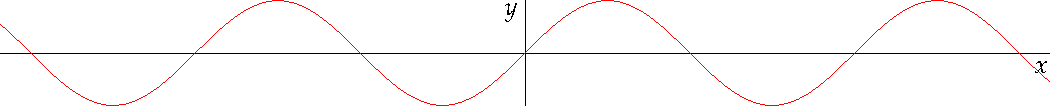
\includegraphics[width=\linewidth]{sine.pdf}
\caption{This graph shows $y = \sin x$ from about $x = [-10, 10]$.
\emph{Notice that this figure takes up the full page width.}}
\label{fig:fullfig}
\end{figure*}

\begin{figure}
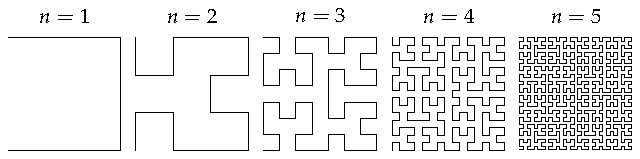
\includegraphics{hilbertcurves.pdf}
\caption[Hilbert curves of various degrees $n$.][6pt]{Hilbert curves of various degrees $n$. \emph{Notice that this figure only takes up the main textblock width.}}
\label{fig:textfig}
\end{figure}

As with sidenotes and marginnotes, a caption may sometimes require vertical adjustment. The \doccmddef{caption} command now takes a second optional argument that enables you to do this by providing a dimension \docopt{offset}. You may specify the caption in any one of the following forms:
\begin{docspec}
\doccmd{caption}\{\docarg{long caption}\}\\
\doccmd{caption}[\docarg{short caption}]\{\docarg{long caption}\}\\
\doccmd{caption}[][\docopt{offset}]\{\docarg{long caption}\}\\
\doccmd{caption}[\docarg{short caption}][\docopt{offset}]%
\{\docarg{long caption}\}
\end{docspec}
A positive \docopt{offset} will push the caption down the page. The short caption, if provided, is what appears in the list of figures/tables, otherwise the ``long'' caption appears there. Note that although the arguments \docopt{short caption} and \docopt{offset} are both optional, they must be provided in order. Thus, to specify an \docopt{offset} without specifying a \docopt{short caption}, you must include the first set of empty brackets \Verb|[]|, which tell \doccmd{caption} to use the default ``long'' caption. As an example, the caption to figure~\ref{fig:textfig} above was given in the form
\begin{docspec}
\doccmd{caption}[Hilbert curves...][6pt]\{Hilbert curves...\}
\end{docspec}

Table~\ref{tab:normaltab} shows table created with the \docpkg{booktabs} package. Notice the lack of vertical rules---they serve only to clutter the table's data.

\begin{table}[ht]
\centering
\fontfamily{ppl}\selectfont
\begin{tabular}{ll}
\toprule
Margin & Length \\
\midrule
Paper width & \unit[8\nicefrac{1}{2}]{inches} \\
Paper height & \unit[11]{inches} \\
Textblock width & \unit[6\nicefrac{1}{2}]{inches} \\
Textblock/sidenote gutter & \unit[\nicefrac{3}{8}]{inches} \\
Sidenote width & \unit[2]{inches} \\
\bottomrule
\end{tabular}
\caption{Here are the dimensions of the various margins used in the Tufte-handout class.}
\label{tab:normaltab}
\end{table}

\newthought{Occasionally} \LaTeX{} will generate an error message:\label{err:too-many-floats}
\begin{docspec}
Error: Too many unprocessed floats
\end{docspec}
\LaTeX{} tries to place floats in the best position on the page. Until it's finished composing the page, however, it won't know where those positions are. If you have a lot of floats on a page (including sidenotes, margin notes, figures, tables, etc.), \LaTeX{} may run out of ``slots'' to keep track of them and will generate the above error.

\LaTeX{} initially allocates 18 slots for storing floats. To work around this limitation, the \TL document classes provide a \doccmddef{morefloats} command that will reserve more slots.

The first time \doccmd{morefloats} is called, it allocates an additional 34 slots. The second time \doccmd{morefloats} is called, it allocates another 26 slots.

The \doccmd{morefloats} command may only be used two times. Calling it a third time will generate an error message. (This is because we can't safely allocate many more floats or \LaTeX{} will run out of memory.)

If, after using the \doccmd{morefloats} command twice, you continue to get the \texttt{Too many unprocessed floats} error, there are a couple things you can do.

The \doccmddef{FloatBarrier} command will immediately process all the floats before typesetting more material. Since \doccmd{FloatBarrier} will start a new paragraph, you should place this command at the beginning or end of a paragraph.

The \doccmddef{clearpage} command will also process the floats before continuing, but instead of starting a new paragraph, it will start a new page.

You can also try moving your floats around a bit: move a figure or table to the next page or reduce the number of sidenotes. (Each sidenote actually uses \emph{two} slots.)

After the floats have placed, \LaTeX{} will mark those slots as unused so they are available for the next page to be composed.

%------------------------------------------------

\section{Captions}
You may notice that the captions are sometimes misaligned. Due to the way \LaTeX's float mechanism works, we can't know for sure where it decided to put a float. Therefore, the \TL document classes provide commands to override the caption position.

\paragraph{Vertical alignment} To override the vertical alignment, use the \doccmd{setfloatalignment} command inside the float environment. For example:

\begin{fullwidth}
\begin{docspec}
\textbackslash begin\{figure\}[btp]\\
\qquad \textbackslash includegraphics\{sinewave\}\\
\qquad \textbackslash caption\{This is an example of a sine wave.\}\\
\qquad \textbackslash label\{fig:sinewave\}\\
\qquad \hlred{\textbackslash setfloatalignment\{b\}\% forces caption to be bottom-aligned}\\
\textbackslash end\{figure\}
\end{docspec}
\end{fullwidth}

\noindent The syntax of the \doccmddef{setfloatalignment} command is:

\begin{docspec}
\doccmd{setfloatalignment}\{\docopt{pos}\}
\end{docspec}

\noindent where \docopt{pos} can be either \texttt{b} for bottom-aligned captions, or \texttt{t} for top-aligned captions.

\paragraph{Horizontal alignment}\label{par:overriding-horizontal}
To override the horizontal alignment, use either the \doccmd{forceversofloat} or the \doccmd{forcerectofloat} command inside of the float environment. For example:

\begin{fullwidth}
\begin{docspec}
\textbackslash begin\{figure\}[btp]\\
\qquad \textbackslash includegraphics\{sinewave\}\\
\qquad \textbackslash caption\{This is an example of a sine wave.\}\\
\qquad \textbackslash label\{fig:sinewave\}\\
\qquad \hlred{\textbackslash forceversofloat\% forces caption to be set to the left of the float}\\
\textbackslash end\{figure\}
\end{docspec}
\end{fullwidth}

The \doccmddef{forceversofloat} command causes the algorithm to assume the float has been placed on a verso page---that is, a page on the left side of a two-page spread. Conversely, the \doccmddef{forcerectofloat} command causes the algorithm to assume the float has been placed on a recto page---that is, a page on the right side of a two-page spread.

%------------------------------------------------

\section{Full-width text blocks}

In addition to the new float types, there is a \docenvdef{fullwidth} environment that stretches across the main text block and the sidenotes area.

\begin{Verbatim}
\begin{fullwidth}
Lorem ipsum dolor sit amet...
\end{fullwidth}
\end{Verbatim}

\begin{fullwidth}
\small\itshape\lipsum[1]
\end{fullwidth}

%------------------------------------------------

\section{Typography}\label{sec:typography}

\subsection{Typefaces}\label{sec:typefaces}\index{typefaces}
If the Palatino, \textsf{Helvetica}, and \texttt{Bera Mono} typefaces are installed, this style will use them automatically. Otherwise, we'll fall back on the Computer Modern typefaces.

\subsection{Letterspacing}\label{sec:letterspacing}
This document class includes two new commands and some improvements on existing commands for letterspacing.

When setting strings of \allcaps{ALL CAPS} or \smallcaps{small caps}, the letter\-spacing---that is, the spacing between the letters---should be increased slightly.\cite{Bringhurst2005} The \doccmddef{allcaps} command has proper letterspacing for strings of \allcaps{FULL CAPITAL LETTERS}, and the \doccmddef{smallcaps} command has letterspacing for \smallcaps{small capital letters}. These commands will also automatically convert the case of the text to upper- or lowercase, respectively.

The \doccmddef{textsc} command has also been redefined to include letterspacing. The case of the \doccmd{textsc} argument is left as is, however. This allows one to use both uppercase and lowercase letters: \textsc{The Initial Letters Of The Words In This Sentence Are Capitalized.}

%------------------------------------------------

\section{Document Class Options}\label{sec:options}

\index{class options|(}
The \doccls{tufte-book} class is based on the \LaTeX\ \doccls{book} document class. Therefore, you can pass any of the typical book options. There are a few options that are specific to the \doccls{tufte-book} document class, however.

The \docclsoptdef{a4paper} option will set the paper size to \smallcaps{A4} instead of the default \smallcaps{US} letter size.

The \docclsoptdef{sfsidenotes} option will set the sidenotes and title block in a \textsf{sans serif} typeface instead of the default roman.

The \docclsoptdef{twoside} option will modify the running heads so that the page number is printed on the outside edge (as opposed to always printing the page number on the right-side edge in \docclsoptdef{oneside} mode). 

The \docclsoptdef{symmetric} option typesets the sidenotes on the outside edge of the page. This is how books are traditionally printed, but is contrary to Tufte's book design which sets the sidenotes on the right side of the page. This option implicitly sets the \docclsopt{twoside} option.

The \docclsoptdef{justified} option sets all the text fully justified (flush left and right). The default is to set the text ragged right. The body text of Tufte's books are set ragged right. This prevents needless hyphenation and makes it easier to read the text in the slightly narrower column.

The \docclsoptdef{bidi} option loads the \docpkg{bidi} package which is used with \tXeLaTeX\ to typeset bi-directional text. Since the \docpkg{bidi} package needs to be loaded before the sidenotes and cite commands are defined, it can't be loaded in the document preamble.

The \docclsoptdef{debug} option causes the \TL classes to output debug information to the log file which is useful in troubleshooting bugs. It will also cause the graphics to be replaced by outlines.

The \docclsoptdef{nofonts} option prevents the \TL classes from automatically loading the Palatino and Helvetica typefaces. You should use this option if you wish to load your own fonts. If you're using \tXeLaTeX, this option is implied (\ie, the Palatino and Helvetica fonts aren't loaded if you use \tXeLaTeX). 

The \docclsoptdef{nols} option inhibits the letterspacing code. The \TL\ classes try to load the appropriate letterspacing package (either pdf\TeX's \docpkg{letterspace} package or the \docpkg{soul} package). If you're using \tXeLaTeX\ with \docpkg{fontenc}, however, you should configure your own letterspacing. 

The \docclsoptdef{notitlepage} option causes \doccmd{maketitle} to generate a title block instead of a title page. The \doccls{book} class defaults to a title page and the \doccls{handout} class defaults to the title block. There is an analogous \docclsoptdef{titlepage} option that forces \doccmd{maketitle} to generate a full title page instead of the title block.

The \docclsoptdef{notoc} option suppresses \TL's custom table of contents (\textsc{toc}) design. The current \textsc{toc} design only shows unnumbered chapter titles; it doesn't show sections or subsections. The \docclsopt{notoc} option will revert to \LaTeX's \textsc{toc} design.

The \docclsoptdef{nohyper} option prevents the \docpkg{hyperref} package from being loaded. The default is to load the \docpkg{hyperref} package and use the \doccmd{title} and \doccmd{author} contents as metadata for the generated \textsc{pdf}.

\index{class options|)}
